%!TEX root = ../../report.tex
\chapter{Experimental framework} % (fold)
\label{cha:experiments}

\section{The test bench} % (fold)
\label{sec:the_test_bench}
During the simulation chapter \ref{cha:simulation}, some tools were created along with the robot in order to carry out specific experiments.
In that case the robot was restricted to a planar movement through the use of a rotational holder with an arm long enough to consider the trajectories as straight.
This experimental setup was inspired by the already existing setup utilized with DACbot in the LPZ Robots simulator.
However, in reality the rotational holder built for the DACbot robot was not an option for RuBi due to its dimensions bigger dimensions.
A new designed was then implemented in conjunction with the existing treadmill used for locomotion experimentation.
Thus, an equivalent structure that could allow the same restrictions as in the simulation over the treadmill was designed and constructed.

The result consists of a frame made out of a set of 3D printed parts and standard components, such as Bosch profiles and carbon fiber tubes.
It is configured to permit RuBi only two degrees of freedom of combined rotation and vertical displacement on its sagital plane.
These two DoF, together with the relative motion provided by the treadmill allow for a full simulation of straight 2D motion.
Besides, the rotation angle can be locked to a specific inclination to constraint the motion to vertical displacements.
This feature was implemented to ease the experimentation on hopping dynamics explained in \ref{sec:vertical_jump_experimentation}.
In the figures \ref{fig:photo_structure} and \ref{fig:legs_structure}, a render and a photo of the real structure are presented.

\begin{figure}[ht!]
    \centering
    \begin{subfigure}[b]{0.49\textwidth}
        \includegraphics[width=\textwidth]{figures/photo_structure}
        \caption{RuBi on the assembled test bench}
        \label{fig:photo_structure}
    \end{subfigure}
    \begin{subfigure}[b]{0.49\textwidth}
        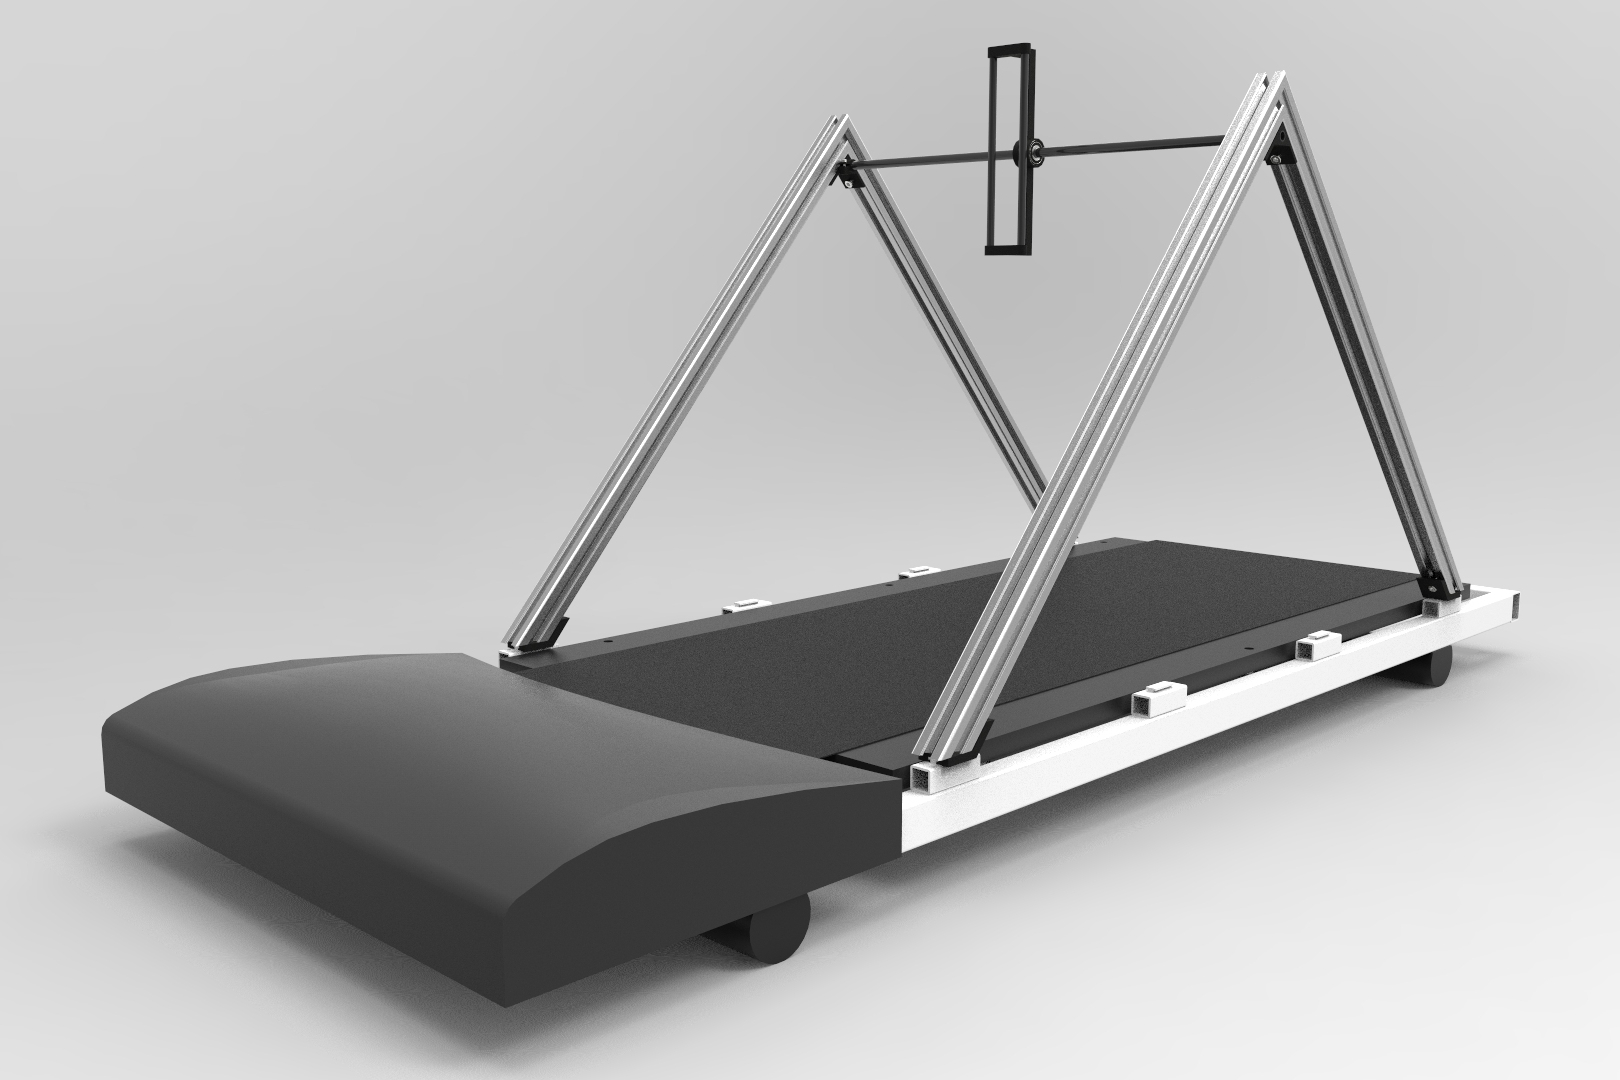
\includegraphics[width=\textwidth]{figures/legs_structure}
        \caption{Original render of the test bench}
        \label{fig:legs_structure}
    \end{subfigure}
\end{figure}  

% section the_test_bench (end)


\section{Vertical jump experimentation} % (fold)
\label{sec:vertical_jump_experimentation}
The theoretical framework presented in \ref{cha:mathematical_model} to develop the formulas used to gauge the requirements of the actuators in \ref{sub:electric_actuators} was meant to be tested empirically in order to assess its viability.
However, the delays suffered in the delivery of some of the components for the prototype, explained in \ref{sec:providers},
together with the other eventualities described in previous chapters prevented from carrying out the devised experiments.

\subsubsection{Experiment 1} % (fold)
\label{ssub:experiment_1}
The jump analysis and dynamic model studied in \ref{sec:jumping_case} and \ref{sec_dynamic_model} could be tested implementing springs stiff enough to model direct transmission and making the robot perform series of vertical jumps on one leg.
To do so, the output of a fully-simulated jump cycle from the MATLAB controller discussed in \ref{sec_dynamic_controller} would be utilized as the input to the impulse controller created in \ref{ssub:impulse_controller}, and tested in the real prototype on the test bench, constrained to only vertical motion.
If the analyses were correct, there should be a correlation between the measured result of $\Delta h$ for a given jump trajectory and the $\Delta h$ expected.


% subsubsection experiment_1 (end)

\subsubsection{Experiment 2} % (fold)
\label{ssub:experiment_2}
In order to evaluate the influence of the elastic actuators in the jump performance from an energy point of view, instead of using the equations presented in \ref{sec:joint_kinetics}, an experimental approach is presented here.
It is suggested the use of the virtual compliant leg model to shape the energetic contribution of each implemented spring to the energy storage capacity of the system.
This method consists in analyzing the compliance of one leg as if it had only one linear spring from the hip joint to the toes, as shown in Figure \ref{fig:virtual_spring1}.

\begin{figure}[ht!]
    \centering
    \begin{subfigure}[b]{0.25\textwidth}
        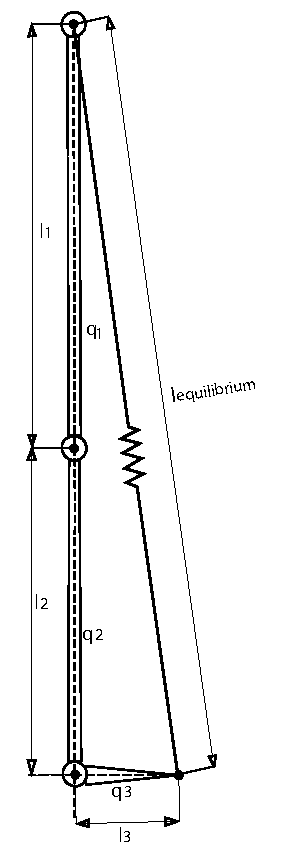
\includegraphics[width=\textwidth]{figures/spring_model_equilibrium.pdf}
        \caption{Virtual spring in equilibrium}
        \label{fig:virtual_spring1}
    \end{subfigure}
    \begin{subfigure}[b]{0.25\textwidth}
        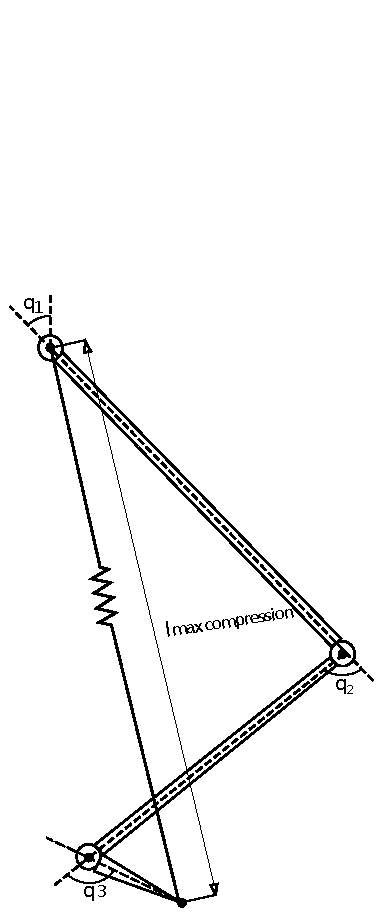
\includegraphics[width=\textwidth]{figures/spring_model_max_compressed.pdf}
        \caption{Virtual spring in max compression}
        \label{fig:virtual_spring2}
    \end{subfigure}
    \begin{subfigure}[b]{0.25\textwidth}
        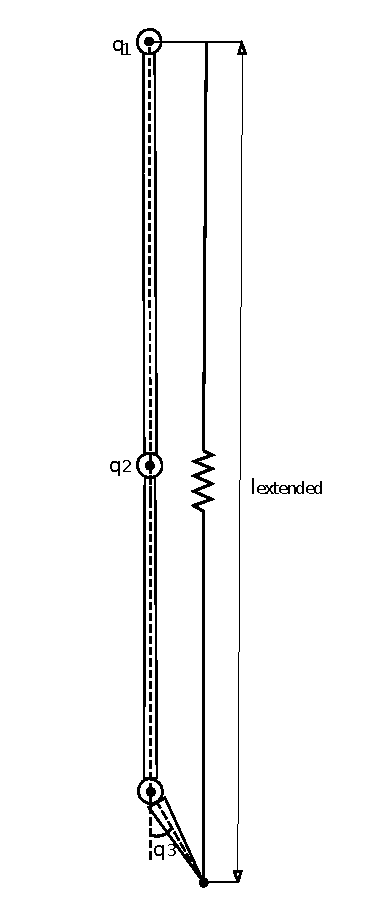
\includegraphics[width=\textwidth]{figures//spring_model_max_extended.pdf}
        \caption{Virtual spring in max extension}
        \label{fig:virtual_spring3}
    \end{subfigure}
\end{figure}  

The energy stored by this linear spring can be decomposed as the sum of the quantities stored by each spring on the leg, as shown in \ref{eq:eq_spring}.
Where $\Delta l_{eq}$ would be the changes in the length of the virtual spring and the constants of the springs are known.
However, the changes in the state of the spring can be hard to calculate or measure empirically.
An study of the different stages that the energy in the system goes through while dropping the robot on one leg from a known height is suggested instead:
\begin{enumerate}
    \item If the robot is dropped from a know altitude $h_{drop}$ in a certain configuration, that could be considered the equilibrium position of the virtual spring, shown in \ref{fig:virtual_spring1}. 
    At that point, the system would contain a potential energy characterized by the initial height $E_{pot}(h_{drop})$.
    \item The instant after landing for a maximum compression of the springs, right before starting the launching reaction caused by the energy stored, is seen as the maximum compression instant, depicted in \ref{fig:virtual_spring2}. 
    Here, all the potential energy has been stored on the springs or lost in the ground contact and trough system losses very difficult to model or measure, $E_{loss1}$ as internal frictions.
    This change in the energy state in the system is represented as in \ref{eq:energy_flow}.
    \item Finally, the take-off configuration, in \ref{fig:virtual_spring3}, would be the one reached once the springs have released the energy and the maximum acceleration upwards is reached. 
    Once the robot has reached its maximum height $h_{rebound}$ all the energy left in the system, $E_{eq}$, has been converted to potential energy again plus other losses, as in equation \ref{eq:energy_flow}.
\end{enumerate}

\begin{equation}
\label{eq:eq_spring}
    E_{eq} = \frac{1}{2}K_{eq}\Delta l^2_{eq} = \frac{1}{2}K_{knee} \Delta \theta^2_{knee} + \frac{1}{2}K_{ankle} \Delta \theta^2_{ankle}
\end{equation}

\begin{equation}
\label{eq:energy_flow}
    \begin{aligned}
        E_{pot}(h_{drop}) = E_{eq} + E_{loss1}\\
        E_{eq} = mg h_{rebound} + E_{loss2}
    \end{aligned}
\end{equation}

To reduce energy losses in non-vertical displacements, the robot trajectory should be physically constrained.
Within the presented theoretical frame, the energy stored by the virtual spring could be calculated simply by measuring $h_{drop}$ and $h_{rebound}$.
However, the right side of equation \ref{eq:eq_spring} cannot be decoupled.
Instead, the configuration and number of springs for several series of the same experiment could be changed, and their influence on the obtained $E_{eq}$ compared to assess their contribution to the overall energy storage capacity of the leg.
A high-speed vision system to provide the height measurements for the experiment, following the model presented in \cite{hs_vision}, is put forward here for consideration. 

It suggested the use of a position controller for the joints in order to fix the joints positions and create a rigid structure of RuBi.
This kind of controller has not been implemented on the top of the current software interface.
However, its fully implemented in the electronics firmware and can be easily created in ROS Control through the standard HW interface class.
% subsubsection experiment_2 (end)

% section vertical_jump_experimentation (end)

\section{Simulation experiments} % (fold)
\label{sec:simulation_experiments}
In the section \ref{sub:example_controllers}, the developed example controllers were presented.
Among them, the impulse controller was created to provide a set of custom peak torques to the joints and generate impulse motion on the frame.
Although the resulting impulses are not controlled in anyway, they permit a fast look to the order of magnitude of the forces necessary in order to jump.
The controller has only been tested in the simulation and in Figure \ref{fig:gazebo_jumping}, RuBi is shown jumping as a result of the torques applied by the controller.
While a real conclusion of the jumping capabilities of the robot can only be achieved by tests in the real robot, the simulation proves to be useful for conceptual testing of the controllers.

% \begin{table}[tb]
%     \caption{Input parameters for the impulse controller that produce a jump in the robot}
%     \label{tab:impulse_controller_inputs}
%     \centering

%     \begin{tabular}{c|c}
%     \textbf{Parameter} & \textbf{Value} \\
%     \hline
%         Hip's torque & -10 N \\
%     \hline
%         Knee's torque & 10 N \\
%     \hline
%         Ankle's torque & -10 N \\
%     \hline
%         Application time & 0.5 s \\
%     \end{tabular}
% \end{table}

\begin{figure}[ht!]
    \centering
    \begin{subfigure}[b]{0.16\textwidth}
        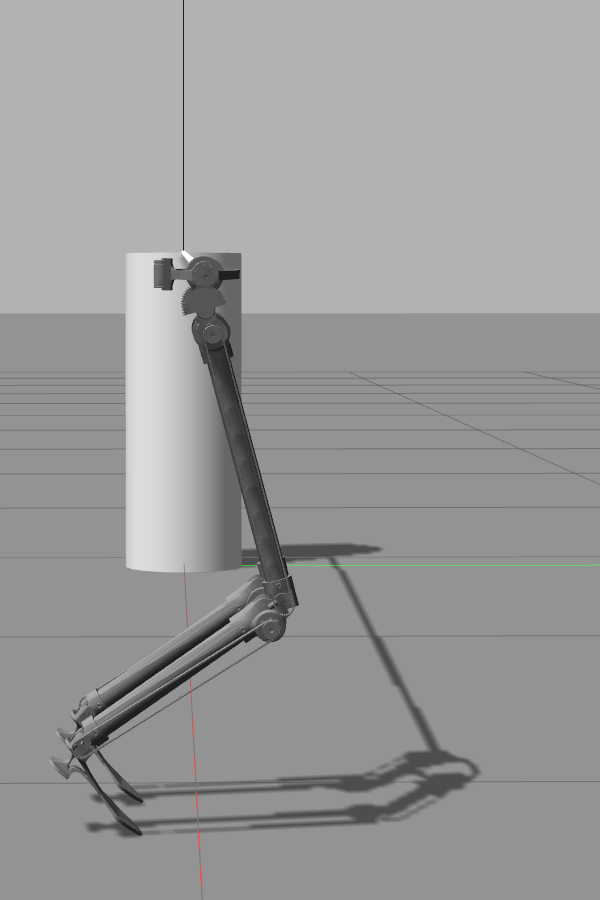
\includegraphics[width=\textwidth]{figures/gazebo_jumping_1}
    \end{subfigure}
    \begin{subfigure}[b]{0.16\textwidth}
        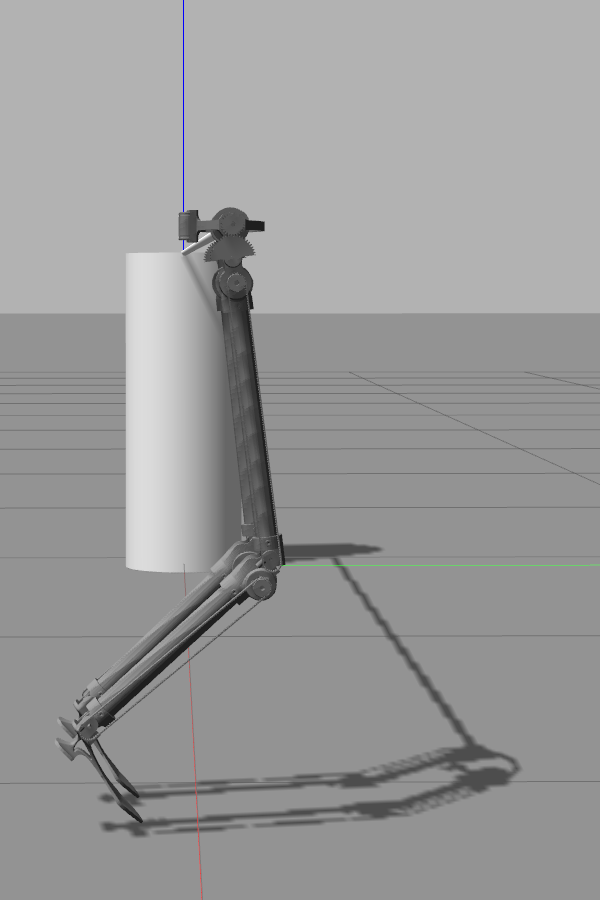
\includegraphics[width=\textwidth]{figures/gazebo_jumping_2}
    \end{subfigure}
    \begin{subfigure}[b]{0.16\textwidth}
        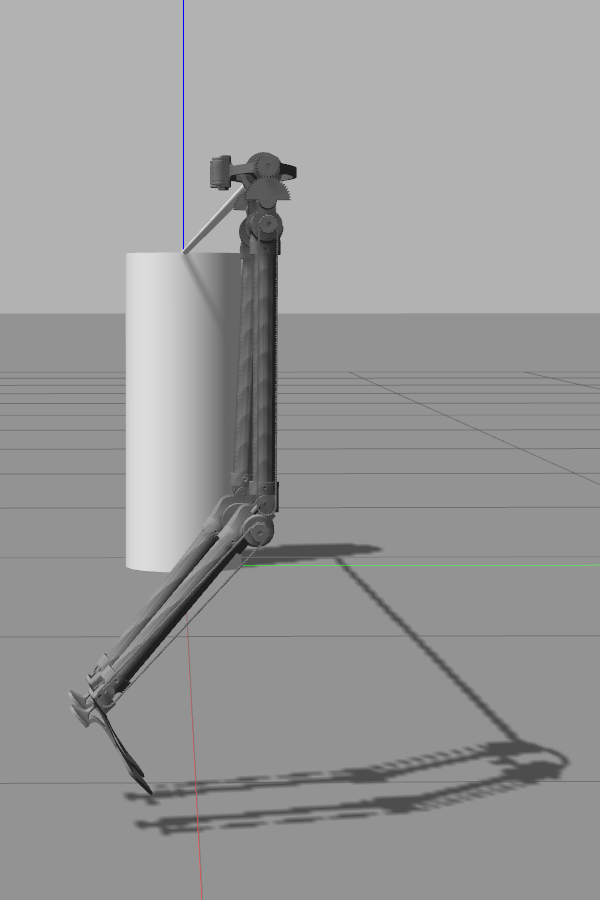
\includegraphics[width=\textwidth]{figures/gazebo_jumping_3}
    \end{subfigure}
    \begin{subfigure}[b]{0.16\textwidth}
        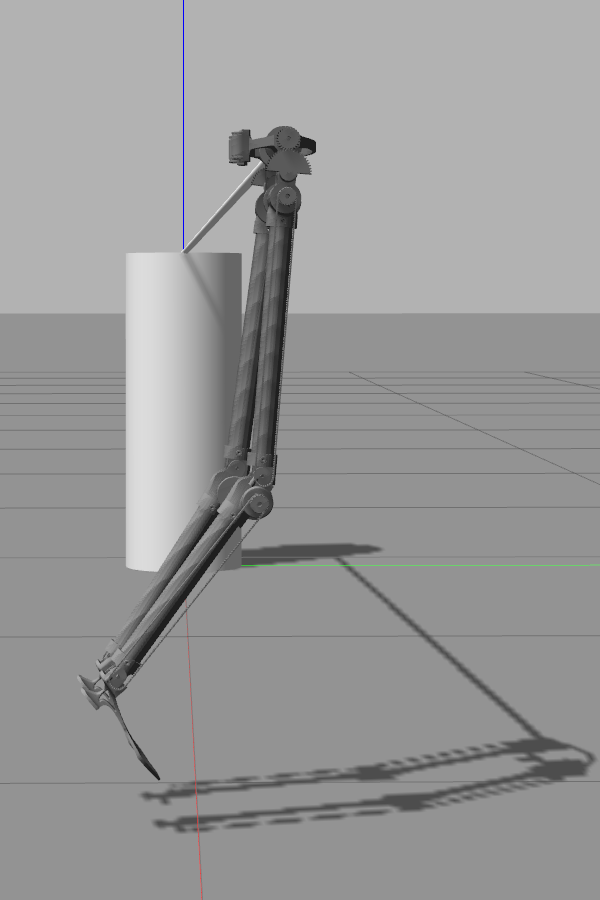
\includegraphics[width=\textwidth]{figures/gazebo_jumping_4}
    \end{subfigure}
    \begin{subfigure}[b]{0.16\textwidth}
        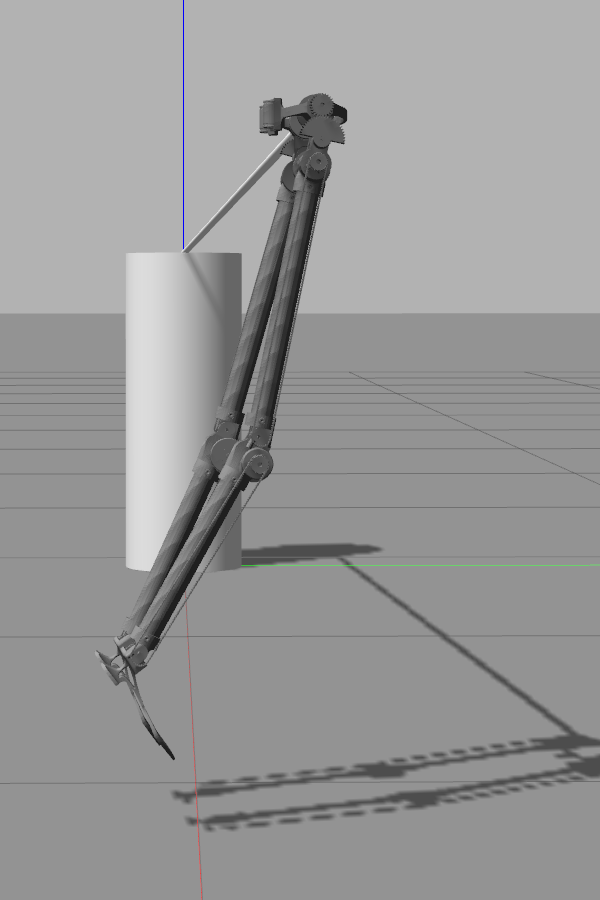
\includegraphics[width=\textwidth]{figures/gazebo_jumping_5}
    \end{subfigure}
    \begin{subfigure}[b]{0.16\textwidth}
        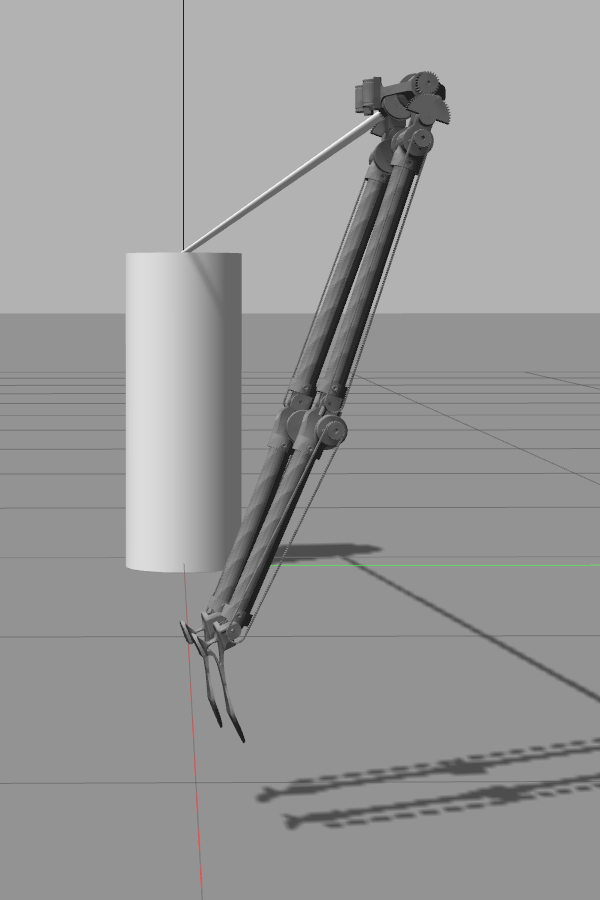
\includegraphics[width=\textwidth]{figures/gazebo_jumping_7}
    \end{subfigure}
    \caption{Screenshots of the robot taken when jumping by using the impulse controller for input torques of $\tau_{ankle}=-10Nm$, $\tau_{knee}=10Nm$, $\tau_{hip}=-10Nm$ during $500 ms$.}
    \label{fig:gazebo_jumping}
\end{figure}    

% section simulation_experiments (end)

% chapter experiments (end)